

\begin{frame}[fragile,label=SubgroupLatticeBasics]{Subgroup Lattice Basics}
Let $U$ and $H$ be subgroups of a finite group.
  \begin{itemize}
  \item<1-> By $UH$ we mean the \emph{set} $\{ u h \mid u\in U, h\in H\}$.\\[6pt]
  \item<2-> $U \join V = \<U,H\>$ means the group generated by $U$ and $H$.\\[6pt]
  \item<3-> $UH \subseteq \<U,H\>$ and 
    equality holds iff $U$ and $H$ permute: 
    \[
    UH = \<U,H\> \quad \Leftrightarrow \quad U H = H U.
    \]
  \end{itemize}
\visible<4->{
\begin{center}
  \begin{tikzpicture}[scale=.4]
    \node (H) at (4,4) [fill,circle,inner sep=\dotsize] {}; \draw (H) node [right] {$H$};
    \node (U) at (-4,4) [fill,circle,inner sep=\dotsize] {}; \draw (U) node [left] {$U$};
    \node (U0) at (0,0) [fill,circle,inner sep=\dotsize] {}; 
    \draw (1.5,-.75) node {$U_0 = U\cap H$};
    \node (UH) at (0,8) [fill,circle,inner sep=\dotsize] {}; \draw (UH) node [above] {$\<U,H\>$};
 \draw
    (U) to [out=-10,in=100] (U0) to [out=170,in=-80] (U)
    (UH) to [out=-10,in=100] (H) to [out=170,in=-80] (UH)
    (H) to [out=190,in=80] (U0) to [out=10,in=-100] (H)
    (UH) to [out=190,in=80] (U) to [out=10,in=-100] (UH);
    \visible<5->{\shade[top color=olivegreen,bottom color=gray!50] 
      (U) to [out=-10,in=100] (U0) to [out=170,in=-80] (U);
      \draw (-7,0) node {$[U_0,U]:=\{V \mid U_0 \leq V \leq U\}$};}
    % \visible<6->{  \shade[top color=blue,bottom color=gray!50] 
    %   (UH) to [out=-10,in=100] (H) to [out=170,in=-80] (UH);
    %   \draw (7,6) node {$[H, \<U,H\>]$};}
    \visible<5->{ \node (V) at (-1.6,1.8) [fill,circle,inner sep=\dotsize] {};
      \draw (-2,2) node {$V$};}
    \end{tikzpicture}
\end{center}
}
\end{frame}


\begin{frame}[fragile,label=IntervalIsomorphisms,shrink=5]{Interval Isomorphisms}
  \begin{columns}
    \begin{column}{0.3\textwidth}
      \begin{center}
        \begin{tikzpicture}[scale=.3]
              \node (H) at (4,4) [draw,circle,inner sep=\dotsize] {}; \draw (H) node [right] {$H$};
    \node (U) at (-4,4) [draw,circle,inner sep=\dotsize] {}; \draw (U) node [left] {$U$};
    \node (U0) at (0,0) [draw,circle,inner sep=\dotsize] {}; 
    \draw (1.5,-.75) node {$U_0 = U\cap H$};
    \node (UH) at (0,8) [draw,circle,inner sep=\dotsize] {}; \draw (UH) node
    [above] {$UH$};
 \draw
    (U) to [out=-10,in=100] (U0) to [out=170,in=-80] (U)
    (UH) to [out=-10,in=100] (H) to [out=170,in=-80] (UH)
    (H) to [out=190,in=80] (U0) to [out=10,in=-100] (H)
    (UH) to [out=190,in=80] (U) to [out=10,in=-100] (UH);

    \visible<1>{\shade[top color=olivegreen,bottom color=gray!-45] 
      (U) to [out=-10,in=100] (U0) to [out=170,in=-80] (U);}
    \visible<4->{
      \fill[color=olivegreen] 
      (U) to [out=-10,in=100] (U0) to [out=170,in=-80] (U);}
    \visible<1,4->{  \shade[top color=olivegreen,bottom color=gray!-45] 
      (UH) to [out=-10,in=100] (H) to [out=170,in=-80] (UH);}
    \visible<5->{\fill[color=orange]    
      (H) to [out=190,in=80] (U0) to [out=10,in=-100] (H);}
    \visible<5->{\shade[top color=orange,bottom color=gray!0]    
      (UH) to [out=190,in=80] (U) to [out=10,in=-100] (UH);}
       \end{tikzpicture}
      \end{center}
    \end{column}
    \begin{column}{0.8\textwidth}
      \begin{itemize}
      \item<1-> If $H\subnormal \<U, H\>$, then %\\[4pt]
        $UH = \<U, H\> \; \text{ and } \; [U_0, U] \cong [H, UH]$.\vskip2mm
        \item<2-> Instead of $H\subnormal \<U,H\>$, assume only
          $UH = \<U,H\>$ and define   
          \begin{equation*}
            %      \label{eq:dedekind-1}
            [U_0, U]^H := \{ V\in [U_0,U] \mid VH = HV\},
          \end{equation*}
          the \alert{$H$-permuting subgroups}.
          \vskip2mm 
        \item<3-> If $U \subnormal UH$,
          define
          \begin{equation*}
            %  \label{eq:dedekind-2}
            [U_0, U]_H := \{ V\in [U_0,U] \mid H\leq N_{UH}(V)\}, 
          \end{equation*}
          the \alert{$H$-invariant subgroups}: 
          $V^h = V \; (\forall h\in H)$.
      \end{itemize}
    \end{column}
  \end{columns}

\vskip4mm

  \visible<4->{
    \begin{lemma}
      \label{lemma-wjd-4}
      \begin{enumerate}
      \item $[H, UH]  \cong  [U_0, U]^H \leq [U_0, U]$ 
       % \only<6>{ and \hskip2mm $[U, UH] \cong  [U_0, H]^U \leq [U_0, H]$.}
\\[6pt]
      \item If $U \subnormal UH$, then  $[U_0, U]_H  = [U_0, U]^H \leq [U_0, U]$.\\[6pt]
      \item If $H \subnormal UH$,  then  $[U_0, U]_H  = [U_0, U]^H = [U_0, U]$.
      \end{enumerate}
    \end{lemma}
}
\note{
  \begin{itemize}
  \item 
  Since $G=UH$ is a group, the hypothesis of (ii) is equivalent to
$H\leq N_G(U)$, and the hypothesis of (iii) is equivalent to $U\leq N_G(H)$.
\item Part (i) of the lemma says that when two subgroups permute, we can
identify the interval above either one of them with the sublattice of
subgroups below the other that permute with the first.
\item Part (ii) is similar except we identify the interval above $H$ with
the  sublattice of $H$-invariant subgroups below $U$.
\item Once we have proved (i), the
proof of (iii) follows trivially from the Noether isomorphism theorem.
  \end{itemize}}

\end{frame}

%%%%%% Example %%%%%%%%%
\begin{frame}[fragile,label=ExampleOfPermutingIso,shrink=5]{Example 1}

  \begin{itemize}
  \item<1-> Consider $G\cong C_3 \times S_3$, say,
    \[G = \<a,b,c \mid a^2, b^3, c^3, [b,a], [c,b], c^{-1}a^{-1}a^c\>\]
\item<2->The subgroups 
\[U = \<a,b\> \cong C_6, \qquad H = \<bc\>\cong C_3\]
permute ($UH = HU$) but neither one normalizes the other.
  \end{itemize}
\vskip4mm
\visible<2->{
\begin{center}
  {\scalefont{.8}
    \begin{tikzpicture}[scale=.4]
      
        \node (U0) at (0,0)  [draw, circle, inner sep=\dotsize] {};
        \draw (U0) node [below] {$U_0 = 1$};
        \node (UH) at (0,8)  [draw, circle, inner sep=\dotsize] {};
        \draw (UH) node [above] {$UH = \<a,b,c\>$};
        \node (V) at (-2.5,2)  [draw, circle, inner sep=\dotsize] {};
        \node (W) at (-.5,3)  [draw, circle, inner sep=\dotsize] {};
        \node (U) at (-3,5)  [draw, circle, inner sep=\dotsize] {};
        \draw (U) node [left] {$U=\<a,b\>$};
        \node (H) at (2.5,3)  [draw, circle, inner sep=\dotsize] {};
        \draw (H) node [right] {$H=\<bc\>$};
        \node (K) at (2,6)  [draw, circle, inner sep=\dotsize] {};

        \draw[semithick] 
        (U0) to (V) to (U) to (W) to (U0) to (H) to (K) to (UH) to (U);
       %\draw (-4.5,2.2) node {$L \cong$};



        \visible<3->{
          \draw (V) node [left] {$\<a\>$};
          \draw (W) node [right] {$\<b\>$};
          \draw (K) node [right] {$\<b,c\>\cong C_3 \times C_3$};
        }
        \visible<4->{\draw[semithick,dotted] (K) to (W);}
    \end{tikzpicture}
  }
\end{center}
}
  \begin{itemize}
  \item<4-> Three of the four subgroups of $U$ permute with $H$.
\\[4pt] As the lemma predicts, $U\cap \<b, c\> = \<b\>$.
  \end{itemize}
\end{frame}


%%%%%% Example2 %%%%%%%%%
\begin{frame}[fragile,label=ExampleOfPermutingIso,shrink=5]{Example 2}

  \begin{itemize}
  \item<1-> The group $S_4$ has subgroups $U\cong D_8$ and $H\cong C_3$ that
    permute but neither one normalizes the other.
  \end{itemize}
\vskip4mm
\visible<2->{
\begin{center}
  {\scalefont{.8}
    \begin{tikzpicture}[scale=.4]
      
        \node (U0) at (0,0)  [draw, circle, inner sep=\dotsize] {};
        \draw (U0) node [below] {$H_0 = 1$};
        \node (UH) at (3,13)  [draw, circle, inner sep=\dotsize] {};
        \draw (UH) node [above] {$HK = S_4$};
        \node (V) at (-3,5)  [draw, circle, inner sep=\dotsize] {};
        \node (W) at (1,5)  [draw, circle, inner sep=\dotsize] {};
        \node (U) at (-2,8)  [draw, circle, inner sep=\dotsize] {};
        \draw (U) node [left] {$H\cong D_8$};
        \node (H) at (5,5)  [draw, circle, inner sep=\dotsize] {};
        \draw (H) node [right] {$K \cong C_3$};
        \node (A4) at (2,10)  [draw, circle, inner sep=\dotsize] {};
        \draw (A4) node [right] {$A_4$};
        \node (S3) at (6,10)  [draw, circle, inner sep=\dotsize] {};
        \draw (S3) node [right] {$S_3$};
        \node (a) at (-3.6,3)  [draw, circle, inner sep=\dotsize] {};
        \node (b) at (-2,3)  [draw, circle, inner sep=\dotsize] {};
        \node (c) at (-1,4)  [draw, circle, inner sep=\dotsize] {};
        \node (d) at (-0,4)  [draw, circle, inner sep=\dotsize] {};
        \node (e) at (-1.5,6)  [draw, circle, inner sep=\dotsize] {};
        \node (f) at (0,6)  [draw, circle, inner sep=\dotsize] {};

        \draw[semithick] 
        (U0) to (a) to (V) to (b) to (U0) to (c) to (V) to (U) to (e) to (c) to
        (f) to (d) to (U0) to (W) to (f) to (U) (UH) to (A4) to (H) to (S3)
        to (UH);
        \draw[semithick,dotted] 
        (U) to (UH)   (U0) to (H);
       %\draw (-4.5,2.2) node {$L \cong$};



      \visible<3->{\draw[semithick,dotted]
        (V) to (A4) (W) to (S3);
        \draw (V) node [left] {$V\cong C_2\times C_2$};
        \draw (W) node [right] {$W\cong C_2 $};
      }
    \end{tikzpicture}
  }
\end{center}
}
\begin{itemize}
\item<2-> Only four subgroups of $U$ permute with $H$%
\visible<3->{, including
    \[ 
U\cap A_4 \cong C_2\times C_2, \qquad U \cap S_3 \cong C_2.
    \]
  }
\end{itemize}
\end{frame}


\begin{frame}[fragile,label=Dedekind]{}
%\vskip-1cm
%The proof relies on Dedekind's modular law for subgroups.
\vskip3mm
\begin{theorem}[Dedekind's Rule]
  \label{lemma-dedekind}
Let $A, B, C$ be subgroups of $G$ with $A\leq B$.  Then,
\[
A(C\cap B) = AC \cap B \quad \text{ and }
\quad (C\cap B)A = CA \cap B.
\]
\end{theorem}
\vskip3mm
In other words, no pentagons.
\vskip3mm
\hfill    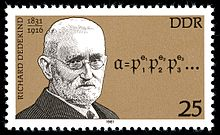
\includegraphics[height=25mm]{Dedekind-stamp}
\note{Draw picture of $N_5$ with $A\leq B$ to demonstrate that it contradicts Dedekind's rule.}
\end{frame}


\begin{frame}[fragile,label=ProofOfIntervalIsomorphism,shrink=5]{Proof of Interval Isomorphism Lemma}
  \begin{columns}
    \begin{column}{0.45\textwidth}
      \begin{claim}[1]
      $[H, UH]  \cong  [U_0, U]^H$ via
        \begin{align*}
          \phi: \;& [H, UH] \ni X \mapsto U\cap X \in [U_0, U]^H\\[6pt]
          \psi: \;& [U_0, U]^H \ni V \mapsto VH \in [H, UH].
        \end{align*}
      \end{claim}
    \end{column}
    \begin{column}{0.55\textwidth}
      \begin{center}
        {\scalefont{.75}
          \begin{tikzpicture}[scale=.35]
                \node (H) at (4,4) [draw,circle,inner sep=\dotsize] {}; \draw (H) node [right] {$H$};
    \node (U) at (-4,4) [draw,circle,inner sep=\dotsize] {}; \draw (U) node [left] {$U$};
    \node (U0) at (0,0) [draw,circle,inner sep=\dotsize] {}; 
    \draw (1.5,-.75) node {$U_0 = U\cap H$};
    \node (UH) at (0,8) [draw,circle,inner sep=\dotsize] {}; \draw (UH) node
    [above] {$UH$};
 \draw
    (U) to [out=-10,in=100] (U0) to [out=170,in=-80] (U)
    (UH) to [out=-10,in=100] (H) to [out=170,in=-80] (UH)
    (H) to [out=190,in=80] (U0) to [out=10,in=-100] (H)
    (UH) to [out=190,in=80] (U) to [out=10,in=-100] (UH);

            \fill[color=olivegreen] 
            (U) to [out=-10,in=100] (U0) to [out=170,in=-80] (U);
            \shade[top color=olivegreen,bottom color=gray!-45] 
            (UH) to [out=-10,in=100] (H) to [out=170,in=-80] (UH);
            \node (V) at (-2.3,2.5) [fill,circle,inner sep=\dotsize] {}; \draw (V) node [left] {$V$};
            \node (VH) at (1.7,6.5){};
            \node (X) at (2.5,5.3) [fill,circle,inner sep=\dotsize] {}; \draw (X) node [right] {$X$};
            \node (UcapX) at (-1.5,1.3){};
            \draw[semithick,dotted] 
            (V) to [out=65,in=-155] (VH)
            (X) to [out=-155,in=65] (UcapX);
          \end{tikzpicture}
        }
      \end{center}
    \end{column}
  \end{columns}
\vskip5mm
  %% \begin{columns}
  %%   \begin{column}{0.6\textwidth}
      \begin{proof}
        \begin{itemize}
        \item[1.] For $X\in [H, UH]$,
          check $U\cap X \in [U_0, U]^H$ by Dedekind's rule.\vskip6pt
        \item[2.] For $V\in [U_0, U]^H$, $VH$ is a group in $[H, UH]$.\vskip6pt
        \item[3.]  Check $\psi \phi$ and $\phi \psi$ are the identity maps. \vskip6pt
        \item[4.] Check $\phi$ and $\psi$ are order preserving.
        \end{itemize}
      \end{proof}

\end{frame}
%% \begin{frame}[fragile,label=ProofOfIntervalIsomorphism,shrink=5]{Proof of Interval Isomorphism Lemma}
%%         \begin{computations}
%%       \begin{itemize}
%%       \item[1.] $(U\cap X) H = UH \cap X= HU \cap X = H(U \cap X)$\vskip10pt
%%       \item[3.] $\psi \phi (X) = (U\cap X)H =UH \cap X = X.$\\[4pt]
%%         $\phi \psi(V)= VH \cap U =V(H\cap U)= V$.\vskip10pt
%%       \item[4.] $X\leq Y \; \Rightarrow \; U\cap X \leq U\cap Y$\\[4pt]
%%         $V\leq W \; \Rightarrow \; VH \leq WH$.
%%       \end{itemize}
%%         \end{computations}
%% \end{frame}

%%% Prezi version %%%
\begin{frame}[fragile,label=ComputationsForProofOfIntervalIsomorphism,shrink=5]{}
 $(U\cap X) H = UH \cap X= HU \cap X = H(U \cap X)$
\end{frame}
\begin{frame}[fragile,label=ComputationsForProofOfIntervalIsomorphism,shrink=5]{}
  $\psi \phi (X) = (U\cap X)H =UH \cap X = X$\\[4pt]
  $\phi \psi(V)= VH \cap U =V(H\cap U)= V$
\end{frame}
\begin{frame}[fragile,label=ComputationsForProofOfIntervalIsomorphism,shrink=5]{}
$X\leq Y \; \Rightarrow \; U\cap X \leq U\cap Y$\\[4pt]
  $V\leq W \; \Rightarrow \; VH \leq WH$.
\end{frame}


      %% \item<1-> 

      %% {\bf Claim 1:} $[H, UH]  \cong  [U_0, U]^H \leq [U_0, U]$.

\begin{frame}[fragile,label=ProofOfIntervalIsomorphism,shrink=5]{Proof of Interval Isomorphism Lemma}
  \begin{columns}
    \begin{column}{0.45\textwidth}
      \begin{claim}[2]
      $[U_0, U]^H$ is a sublattice of $[U_0,U]$.
      \end{claim}
    \end{column}
    \begin{column}{0.55\textwidth}
       \begin{center}
        {\scalefont{.8}
          \begin{tikzpicture}[scale=.35]
                \node (H) at (4,4) [draw,circle,inner sep=\dotsize] {}; \draw (H) node [right] {$H$};
    \node (U) at (-4,4) [draw,circle,inner sep=\dotsize] {}; \draw (U) node [left] {$U$};
    \node (U0) at (0,0) [draw,circle,inner sep=\dotsize] {}; 
    \draw (1.5,-.75) node {$U_0 = U\cap H$};
    \node (UH) at (0,8) [draw,circle,inner sep=\dotsize] {}; \draw (UH) node
    [above] {$UH$};
 \draw
    (U) to [out=-10,in=100] (U0) to [out=170,in=-80] (U)
    (UH) to [out=-10,in=100] (H) to [out=170,in=-80] (UH)
    (H) to [out=190,in=80] (U0) to [out=10,in=-100] (H)
    (UH) to [out=190,in=80] (U) to [out=10,in=-100] (UH);

            \fill[color=olivegreen] 
            (U) to [out=-10,in=100] (U0) to [out=170,in=-80] (U);
            \shade[top color=olivegreen,bottom color=gray!-45] 
            (UH) to [out=-10,in=100] (H) to [out=170,in=-80] (UH);
            \node (V) at (-2.3,1.7) [fill,circle,inner sep=\dotsize] {};
            \draw (V) node [left] {$V$};
            \node (W) at (-1.5,2)[fill,circle,inner sep=\dotsize] {};
            \draw (W) node [right] {$W$};
          \end{tikzpicture}
        }
      \end{center}
 %     \vskip1cm
    \end{column}
  \end{columns}
       \begin{proof}
          Fix $V, W \in [U_0, U]^H$.\vskip6pt
          \begin{itemize}
          \item[1.] Check $V \join W = \<V, W\>$ permutes with $H$. (easy)\vskip10pt
          \item[2.]Check $V \cap W$ permutes with $H$.
          \end{itemize}
          \end{proof}
%% To prove (ii), assuming $U\subnormal G$, we show that if $U_0 \leq V \leq U$,
%% then $VH = HV$ if and only if $H\leq N_G(V)$.
%% If $H\leq N_G(V)$, then $VH = HV$ (even when $U \notsubnormal G$).
%% Suppose $VH = HV$.  We must show $(\forall v\in V)\, (\forall h\in H)\; hvh^{-1}\in
%% V$.  Fix $v\in V, \, h\in H$.  Then, $hv = v'h'$ for some $v'\in V,\, h'\in H$, since
%% $VH = HV$.  Therefore, $v' h' h^{-1} = hvh^{-1} = u$ for some $u\in U$, since
%% $H\leq N_G(U)$. This proves that $hvh^{-1}\in VH\cap U = V(H\cap U) = VU_0 = V$, as
%% desired.
 
\end{frame}

%% \begin{frame}[fragile,label=ProofOfIntervalIsomorphism,shrink=5]{Proof of Interval Isomorphism Lemma}
%%         \begin{computations}
%%       \begin{itemize}
%%       \item[2.] Fix $x \in V \cap W$ and $h\in H$.\\[6pt]  
%%           {\bf To Show:} $xh = h'x'$ for some $h'\in H, \, x'\in V\cap W$.\\[6pt]
%%           Since $V$ and $W$ permute with $H$, 
%%           \[xh = h_1 v \quad \text{ and } \quad xh = h_2 w\]
%%           for some $h_i\in H,\,v \in V,\, w \in W$.\\[10pt]
%%           {\bf Exercise:} Check that this puts $v\in V \cap HW \leq V \cap W$. 
%%           \note{
%%             \[h_1 v = h_2 w \;\Rightarrow \; v = h_1^{-1}h_2 w \in HW.\]
%%             So $v\in V \cap HW$, which is below $V$ and
%%             $U\cap HW = \phi \psi(W) = W$.  
%%             \[\therefore \quad v \in V \cap HW \leq V \cap W.\]
%%             which proves $xh = h_1 v$ for $h_1\in H$ and $v \in V\cap W$, as
%%             desired.}
%%       \end{itemize}
%%         \end{computations}
%% \end{frame}

%%% Prezi version %%%
\begin{frame}[fragile,label=ComputationsForProofOfIntervalIsomorphism,shrink=5]{}
      Fix $x \in V \cap W$ and $h\in H$.\\[6pt]  
      {\bf To Show:} $xh = h'x'$ for some $h'\in H, \, x'\in V\cap W$.
\end{frame}
\begin{frame}[fragile,label=ComputationsForProofOfIntervalIsomorphism,shrink=5]{}
          Since $V$ and $W$ permute with $H$, 
          \[xh = h_1 v \quad \text{ and } \quad xh = h_2 w\]
          for some $h_i\in H,\,v \in V,\, w \in W$.
\end{frame}
\begin{frame}[fragile,label=ComputationsForProofOfIntervalIsomorphism,shrink=5]{}
          {\bf Exercise:} Check that this puts $v\in V \cap HW \leq V \cap W$. 
\end{frame}
\begin{frame}[fragile,label=ComputationsForProofOfIntervalIsomorphism,shrink=5]{}
            \[h_1 v = h_2 w \;\Rightarrow \; v = h_1^{-1}h_2 w \in HW.\]
            So $v\in V \cap HW$, which is below $V$ and
            $U\cap HW = \phi \psi(W) = W$.  
            \[\therefore \quad v \in V \cap HW \leq V \cap W.\]
            which proves $xh = h_1 v$ for $h_1\in H$ and $v \in V\cap W$, as
            desired.
\end{frame}

\begin{frame}[fragile,label=L7second,shrink=5]{}
  \begin{center}
    {\scalefont{.75}
      \begin{tikzpicture}[scale=.7]
              \node (J1) at (0,1)  [draw, circle, inner sep=\dotsize] {};
      \draw (.36, 1) node {$J_1$};
      \node (H) at (1,0)  [draw, circle, inner sep=\dotsize] {};
      \draw (1.16, -.2) node {$H$};
      \node (M2) at (1,2)  [draw, circle, inner sep=\dotsize] {};
      \draw (1.4, 2) node {$M_2$};
      \node (J2) at (2,1)  [draw, circle, inner sep=\dotsize] {};
      \draw (2.2, .8) node {$J_2$};
      \node (G) at (2,3)  [draw, circle, inner sep=\dotsize] {};
      \draw (2.3, 3.1) node {$G$};
      \node (M1) at (3,2)  [draw, circle, inner sep=\dotsize] {};
      \draw (3.35, 2) node {$M_1$};
      \node (K) at (-1,1.2)  [draw, circle, inner sep=\dotsize] {};
      \draw (-1.28, 1.15) node {$K$};

      \draw[semithick] (H) to (J1) to (M2) to (G) to (M1) to (J2) to (H) (J2) to (M2);
      \draw[semithick] (H) to (K) to (G);

      \end{tikzpicture}
    }
  \end{center}

\begin{theorem}
\label{thm:except-seven-elem}
Suppose $H<G$, $\core_G(H) = 1$, and 
$L_7 \cong [H,G]$.  Then
\begin{enumerate}[(i)]
\item<1-> $G$ is a primitive permutation group.
\item<1-> If $N\ssubnormal G$, then $C_G(N) = 1$.
\item<1-> $G$ contains no non-trivial abelian normal subgroup.
\item<1-> $G$ is not solvable.
\item<1-> $G$ is subdirectly irreducible.
\item<1-> With the possible exception of at most one maximal subgroup, $M_1$ or $M_2$,
  all proper subgroups in the interval $[H,G]$ are core-free. 

%% The three subgroups in $[H,G]$ which cover $H$ (the atoms) are
%%   core-free.  At least one two of the three maximal subgroups (the co-atoms) in
%%   the interval are core-free. 
\end{enumerate}
\end{theorem}
%% \note{  It is obvious that 
%%   \begin{itemize}
%%   \item (ii) $\Rightarrow$ (iii) $\Rightarrow$ (iv), and  
%% \item (ii) $\Rightarrow$ (v), but we include these for
%%   emphasis;
%% \item the hard work is in proving (ii) and (vi), but
%%   the main goal is the pair of restrictions (iii) and (v), which allow us to rule
%%   out a number of the O'Nan-Scott types describing primitive permutation
%%   groups. 
%%   \end{itemize}}
\end{frame}

\begin{frame}[fragile,label=IdeaOfL7Proof,shrink=5]{Idea of the proof}
    %% \begin{column}{0.3\textwidth}
      \begin{center}
        {\scalefont{.78}
          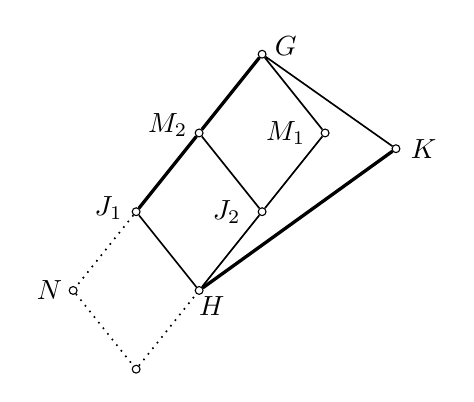
\begin{tikzpicture}[scale=1]
      \node (N) at (-.6,0)  [draw, circle, inner sep=1pt] {};
      \draw (-.9, 0) node {$N$};
      \node (NcapH) at (.2,-1)  [draw, circle, inner sep=1pt] {};
      \node (J1) at (0.2,1)  [draw, circle, inner sep=1pt] {};
      \draw (-.15, 1.05) node {$J_1$};
      \node (H) at (1,0)  [draw, circle, inner sep=1pt] {};
      \draw (1.16, -.2) node {$H$};
      \node (M2) at (1,2)  [draw, circle, inner sep=1pt] {};
      \draw (.6, 2.1) node {$M_2$};
      \node (J2) at (1.8,1)  [draw, circle, inner sep=1pt] {};
      \draw (1.35, 1.) node {$J_2$};
      \node (G) at (1.8,3)  [draw, circle, inner sep=1pt] {};
      \draw (2.1, 3.1) node {$G$};
      \node (M1) at (2.6,2)  [draw, circle, inner sep=1pt] {};
      \draw (2.1, 2) node {$M_1$};
      \node (K) at (3.5,1.8)  [draw, circle, inner sep=1pt] {};
      \draw (3.85, 1.8) node {$K$};
      \draw[semithick,dotted] (J1) to (N) to (NcapH) to (H);
      \visible<4->{\draw[very thick] (J1) to (M2) to (G) (H) to (K);}
      \draw[semithick] (J1) to (M2) to (G) (H) to (K);
      \draw[semithick] (H) to (J1) to (M2) to (G) to (M1) to (J2) to (H) to (K)
      to (G) (J2) to (M2);
    \end{tikzpicture}
 }
\end{center}
      
  %%   \end{column}
  %% \end{columns}

  %% \begin{columns}
  %%   \begin{column}{0.7\textwidth}
      {\bf Claim:} 
      $J_1$ and $J_2$ are core-free subgroups of $G$.\\[6pt]
      {\bf Proof:}
      \begin{itemize}
      \item<2->
      If $N\ssubnormal G$ then $NH$ permutes with each subgroup containing $H$.  
      \note{Let $H \leq X \leq G$.  Then $NHX = NX = XN= XHN = XNH$.}
      \item<3-> If $1\neq N\leq J_1$, then $NH = J_1$, so $J_1$ and $K$ permute.
      \item<4-> Since $J_1K = G$ and $J_1\cap K = H$, our lemma yields
      \[
        [J_1, G] \cong [H, K]^{J_1} = \{X \in[H, K] \mid J_1X=XJ_1 \}.
        \]
   \uncover<5->{Impossible!}
      \end{itemize}

    %% \end{column}


\end{frame}

\begin{frame}[fragile,label=OSTheorem]{}
\vskip2mm
\hskip3mm

\includegraphics[height=30mm]{inputs/Aschbacher3}
\begin{center}

\includegraphics[height=25mm]{inputs/ONan}
\end{center}
\hfill    

\includegraphics[height=28mm]{inputs/Scott}

\end{frame}


\begin{frame}[fragile,label=OSTheorem]{Aschbacher-O'Nan-Scott Theorem}
Let $G$ be a primitive permutation
group of degree $d$, and let $N := \Soc(G) \cong T^m$ with $m \geq 1$. 
Then one of the following holds.
\vskip2mm
\begin{enumerate}
\item 
$N$ is regular and
  \begin{itemize}
  \item 
  \alert{(Affine type)} $T$ is cyclic of order $p$, so $|N| = p^m$ . Then 
$d = p^m$ and $G$ is permutation isomorphic to a subgroup of the affine
general linear group $\AGL(m,p)$.
\vskip2mm
\item \alert{(Twisted wreath product type)} $m \geq 6$, the group $T$ is 
  nonabelian and $G$ is a group of \emph{twisted wreath product type}, with
  $d = |T|^m$.
  \end{itemize}
\vskip2mm
\item $N$ is non-regular, non-abelian, and
  \begin{itemize}
  \item 
\alert{(Almost simple type)} $m = 1$ and $T \leq G \leq \Aut(T)$.
\vskip2mm
\item \alert{(Product action type)} $m \geq 2$ and $G$ is permutation isomorphic to a
subgroup of the product action wreath product $P \wr S_{m/l}$ of degree
$d = nm/l$. The group $P$ is primitive of type 2.(a) or 2.(c), $P$ has
degree $n$ and $\Soc(P) \cong T^l$, where $l \geq 1$ divides $m$.
\vskip2mm
\item 
\alert{(Diagonal type)} $m \geq 2$ and $T^m \leq G \leq T^m . (\Out(T ) \times S_m)$, with
the diagonal action. The degree $d = |T|^{m-1}$.
  \end{itemize}
\end{enumerate}
\end{frame}


\begin{frame}[fragile,label=OSTheoremHistory]{Aschbacher-O'Nan-Scott Theorem}
For some interesting history, see Peter Cameron's blog at 
\begin{center}
{\small  \url{http://cameroncounts.wordpress.com/tag/onan-scott-theorem/}}
\\[8pt]
          
\includegraphics[height=2cm]{inputs/qrCameron}
        \end{center}

\end{frame}

% \begin{frame}[fragile,label=FinalConclusions]{}
%   \begin{center}
%   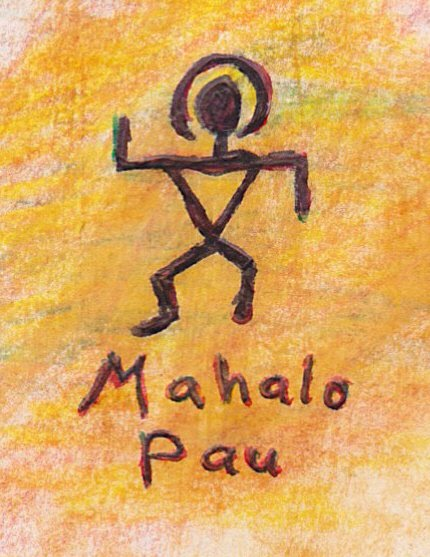
\includegraphics[height=2in]{MahaloPau}
%   \end{center}
% \end{frame}

